\documentclass[spanish,letterpaper,12pt,oneside,openany]{book}
\usepackage[english]{babel}
\usepackage{babelbib}
\usepackage{etoolbox}
\patchcmd\btxselectlanguage{\csname}{\csname TEMPPATCH}{}{} % Para hacer a babelbib funcionar
\usepackage{amstext, amssymb, amsthm, amsmath, amsbsy}
\usepackage{tabularx}
\usepackage[ansinew]{inputenc}
\usepackage[margin=20pt,font=small,labelfont=bf,labelsep=period]{caption}%%Para modificar el formato del texto de los "caption"
\usepackage{graphicx}
\usepackage{url}
\usepackage{listings}%%Para incluir codigo
\usepackage[final]{pdfpages}%%Para incluir archivos en pdf
\usepackage{geometry}
\usepackage{enumerate}
\usepackage{subfig}%%Para incluir subgraficos
\usepackage[pdftex, pdftitle={Finite Element Methods}, pdfauthor={J. Gomez}, pdfsubject={Class Notes}, pdfkeywords={Computational Mechanics, Finite Element Methods}, pdfpagemode=UseOutlines,bookmarks,bookmarksopen,pdfstartview=FitH,colorlinks,linkcolor=blue, urlcolor=black, citecolor=blue]{hyperref} %%Para incluir detalles cucas del pdf
\usepackage[ruled]{algorithm2e}%%Para incluir algoritmos
\usepackage{float}
\usepackage{multirow}
\usepackage{leftidx}
%\usepackage{algorithm2e}
\usepackage{algorithmic}
\usepackage{cite}  %% Para poner bonitas las citas
\usepackage{bookmark} %% Para poder organizar las etiquetas en pdf
\geometry{verbose,letterpaper,tmargin=3cm,bmargin=3cm,lmargin=2cm,rmargin=2cm}
%%%%%%%%%%%%%%%%%%%%%%%%%%%%%%%%%%%%%%%%%%%%%%%%%%%%%%%%%%%%%%%%%%%%%%%%%%%%
%Nuevos Comandos

\setlength{\parskip}{0.5cm}

% Comillas:   ``''

\newcommand{\urlbib}[1]{{\footnotesize{\url{#1}}}} % para incluir urls en las referencias
\newcommand{\fullref}[1]{\ref{#1} de la p\'agina \pageref{#1}}

%%%%%%%%%%%%%%%%%%%%%%%%%%%%%%%%%%%%%%%%%%%%%%%%%%%%%%%%%%%%%%%%%%%%%%%%%%%%
\begin{document}
%%
\renewcommand{\tablename}{Tabla}
\renewcommand{\figurename}{Figura}
\renewcommand{\contentsname}{Table of Contents}
\renewcommand{\listtablename}{Lista de tablas}
\renewcommand{\listfigurename}{Lista de figuras}

%%
%%%%%%%%%%%%%%%%%%%%%%%%%%%%%%%%%%%%%%%%%%%%%%%%%%%%%%%%%%%%%%%%%%%%%%%%%%%%
%%%%%%%%%% Portada %%%%%%%%%%
%Portada
%
\begin{center}
\Large{Class Notes: Introduction to the Finite Element Methods}
\large
\\[30mm]
Juan David G\'omez Cata\~no\\
\emph{jgomezc1@eafit.edu.co}
\\[40mm]
Grupo de Investigacion en Mecanica Aplicada
\\
Civil Engineering Department
\\
School of Engineering
\\
Universidad EAFIT
\\
Medell\'in, Colombia
\\
2013
\end{center}
\thispagestyle{empty}

\frontmatter
%%%%%%%%%%%%%%%%%%%%%%%%%%%%%%%%%%%%%%%%%%%%%%%%%%%%%%%%%%%%%%%%%%%%%%%%%%%%
% Tabla de contenido
\pdfbookmark[0]{Tabla de contenido}{}
\tableofcontents


\mainmatter
%%%%%%%%%%%%%%%%%%%%%%%%%%%%%%%%%%%%%%%%%%%%%%%%%%%%%%%%%%%%%%%%%%%%%%%%%%%%
%%%%%%%%%% Introduccion %%%%%%%%%%
%Seccion "Resumen"
%

\cleardoublepage \phantomsection
\addcontentsline{toc}{chapter}{Summary}
\chapter*{Summary}

\vspace{-1cm}

Class Notes for the Course Introduction to the Finite Element Methods


\textbf{Palabras clave: } Computational Mechanics, Finite Element Methods.

%Chapter "Introduction"
%
\chapter{Introduction}

In an introductory graduate course in the Finite Element Method (FEM), the purpose is to develop a basic understanding of the discrete or numerical strategy of Finite Element-(FE) Algorithms when a closed form solution to a Boundary Value Problem (BVP) is not possible due to complexities existing probably: in the boundary conditions, material behavior or in the kinematic description used in the model. In such a course, in order to master and identify the main mathematical and algorithmic aspects of the method at the beginners level, the studied problem is kept lineal. In this sense 4 key aspects make the core of the introductory course (at least for the case of the linearized theory of elasticity boundary value problem):

\begin{itemize}

\item Formulation and identification of the strong form of the Boundary Value Problem (BVP) where the continuum mechanics governing equations are revisited and particularized to the case of linear elastic material behavior. The BVP is completed by identifying the correct prescription of boundary conditions for a well posed mathematical problem.

\item Formulation and identification of the weak form of the BVP where the governing equations and natural boundary conditions representing equilibrium at the material point level are replaced by an equivalent but weaker form of equilibrium now valid at the global level.  In the case of a Continuum Mechanics problem this so-called weak form can be shown to be equivalent to the principle of virtual power and lends itself for the partition of the problem into sub-domains or finite size elements.

\item Introduction of the idea of discretization dividing the problem into subdomains and using interpolation theory within each subdomain-In the context of the FE method this is the subject of shape functions. Once the computational specimen has been divided into subdomains (or a mesh of finite elements) the selected primary variable is approximated within each element via interpolation of the known response at selected predefined points or nodes.

\item Computational aspects grouped also into 5 points:
	\begin{itemize}
	\item Formulation of elemental matrices in the physical space.
	\item Formulation of elemental matrices in the natural domain-Isoparametric transformation.
	\item Numerical integration: Gauss quadrature.
	\item Assembly of system matrices and imposition of boundary conditions.
	\item Solution of the discrete equilibrium statement and calculation of elemental results.
	\end{itemize}
\end{itemize}

These 4 key points are perfectly well documented in numerous nicely written textbooks and it could be argued that is not even worth to register for an introductory course since a moderately dedicated student can accomplish the task via self-study. Unfortunately, linearity is scarce--although useful to grasp the basic understanding of the problem--and the real world is full of non-linear behavior and understanding the needed algorithms can be easily justified. In this \todo{Check name of the ```course".}\textcolor{red}{Advanced Finite Element Methods course} the goal is then to understand the basic aspects of non-linear finite element analysis.  Like in the linear case there is also a vast amount of literature for the non-linear problem.  However, in the non-linear case the kinematic problem itself may take different routes leading to a wide variety of FEM formulations that will difficult a self-study strategy.  Considering the above this brief set of class notes is intended as a guide for self-study and more important represents a help towards the implementation of the algorithm for the consideration of Material and Geometric Non-linearities in Solids.

The basic reference is Professor Bathe's textbook \cite{book:bathe} but we will also follow closely ABAQUS Theory Manual \cite{abaqus_theory}. ABAQUS is a multi-physics oriented commercially available finite element analysis tool. Its strength resides in the effective non-linear algorithms and on the capability of taking user subroutines written in Fortran or in \CPP.  The possibility of implementing user subroutines makes it a very powerful research tool.  In the particular case of a stress/displacement analysis problem with non-linearities these are considered through the kinematics contribution or through the material contribution.  In the first case the non-linear behavior must be considered at the element level while in the second it corresponds to the response of a material point which in the context of the FEM algorithm corresponds to an integration point. In ABAQUS those two sources of non-linearity can be independently controlled by the user via user subroutines UEL and UMAT.  In both cases the non-linearity is primarily solved by the classical Newton-Raphson scheme and that will be the approached followed herein.  Although the notes are mainly written for an advanced course the specific problem of a linear solid usually studied in the introductory course can be derived like a particular case of the most general non-linear algorithm.

The current set of Class Notes is organized as follows.  First and since we will be dealing with history dependent non-linear problems the most powerful (at least when it works) solution algorithm, namely the Newton-Raphson iteration is studied.  The technique is first illustrated for the simple 1D-case and then generalized into the multi-degree of freedom system.  In both cases pseudo-codes will be presented preparing the way for the Finite Element Algorithm.  The presentation however is not exhaustive in mathematical terms and the reader is referred to excellent treatments like Burden \cite{book:burden2011} and Press et al. \cite{book:numerical_recipes} for the mathematical aspects of the Newton method.

In the next section the briefly introduced Newton-Raphson technique is contextualized to the case of a system of equations representing equilibrium between internal and external forces as typically found in a finite element model.  Moreover, the non-linearities come into play through a dependence of the internal forces into displacements.  At this stage the details of the formulation of the finite element equations via discretization into nodal variables is not presented but emphasis is laid down into the solution algorithm.  Interest is then given to the particular form taken by the Newton-Raphson algorithm into the commercial finite element code ABAQUS.  That code can be used as a powerful non-linear equation solver where the coefficient matrix and the excitation can be directly controlled by the user.  Moreover the solver can be used into a multi-physics context in terms of generalized forces and fluxes.  In the particular case of the stress analysis finite element method the user can control the elemental contribution to the coefficient matrix and the contribution of each material point to obtain that element contribution.  This is achieved through the so-called user subroutines UEL  for element and UMAT  for material.  Having introduced the Newton-Raphson method the notes concentrate next on general discretization aspects starting from the physical strong form of the equations in the deformed configuration and passing to an arbitrary weak form in the reference configuration.  The resulting algorithm is therefore a Total Lagrangian (TL) method.  Once the general equations are introduced a particular work conjugate stress-strain pair is chosen and the discrete equations, including kinematic interpolators, are described.

\section*{Notation}
In a non-linear algorithm the bookkeeping is involved since we have to simultaneously record 4 different fields as follows:
\begin{itemize}
	\item The physical fields in terms of tensorial descriptions.
	\item The time field since the problem is solved incrementally 	and time may appear as an artificial chronological variable 	or as a real quantity in a dynamic problem.
	\item The interpolation field.  Since all the involved variables will be interpolated we will need to keep track of the way this interpolation is being performed.
	\item The iterations field needed in the solution of the non-linear problem.
\end{itemize}
In order to keep this bookkeeping simple we use the following indicial notation with subscripts and superscripts

\begin{figure}[h]
\centering
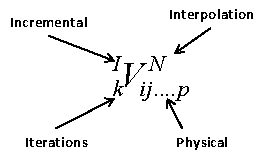
\includegraphics[width=4cm]{img/figure1_1.pdf}
\caption{General notation to study non-linear finite element problems}
\label{fig:notation}
\end{figure}

\todo{Review notation.}Capital superscripts will be reserved for the incremental time description and for the interpolation scheme.  For instance an expression like   refers to the time instant   while   refers to . Similarly a variable   refers to interpolation over the node. Left and right subscripts will be used to make reference to the iteration being performed and the order of the tensor variable.  For instance   refers to a second order tensor corresponding to the iteration.
%Capitulo "Elastodinamica"
%
\chapter{Equilibrium Equations}

\section{General Equilibrium Equations}
In this section we develop the incremental equations needed in a general non-linear problem.  First, geometric non-linearities valid for any stress-strain pair are considered.  Second, focus is shifted towards the particular case of the Second Piola-Kirchoff-Green Lagrange Strain pair.

Let   represent the current (deformed) configuration of a deformable medium with equilibrium equations and boundary conditions

\begin{equation}
{\sigma _{ij,j}} + {f_i} = 0	 
\end{equation}			

\begin{equation}
{t_i} = {\sigma _{ij}}{\hat n_j}
\end{equation}	 		

where   represents the Cauchy definition of stress (or force per unit of deformed surface) and   the corresponding tractions vector at a surface with outward normal  .  In the equilibrium equations stated in (1) the domain   is unknown which makes the problem inherently non-linear.  On the other hand this equilibrium statement is mathematically indeterminate since 9 unknown stress components must be solved out of 6 field equations.  The indeterminacy is destroyed after the problem is kinematically described and connected to the stress field via constitutive modeling which can involve additional sources of non-linearity.  To summarize the problem is non-linear since the domain   is unknown, this is what we typically call a Geometric Non-linearity and will be reflected in the mathematical description of changes in configuration.



\subsection{Lagrangian description of the equilibrium equations}
The conceptual definition of Cauchy stress is the only one useful for the engineer since it describes forces per unit deformed surface.  This validity is clearly identified in the fact that the equilibrium equations stated in (1) have been formulated in the stressed deformed domain   where the body is in fact in equilibrium.  The difficulty associated with the unknown domain may be dealt with in alternative ways.  In the case of a solid body it is convenient to refer everything to the undeformed or reference configuration (with known domain)   and proceed from there using linearization which corresponds to a Total Lagrangian (TL) approach.  It is then useful to understand the transformation of the problem to   via pullback operations.  This process implies the introduction or consideration of mathematically  defined stress definitions and newly developed kinematic descriptions.  In this section we consider such transformations first from a dynamic point of view and later using thermodynamic principles we address the problem of identifying the proper strain measures.
\begin{figure}[h]
\centering
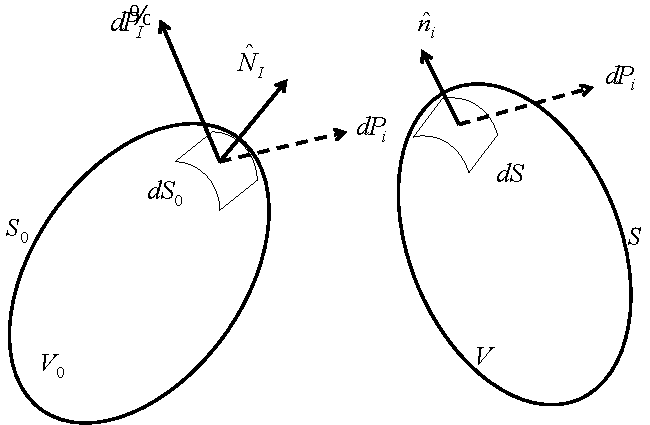
\includegraphics[width=8cm]{img/figure1_2.pdf}
\caption{Definition of the natural domain}
\label{fig:natural domain}
\end{figure}

\subsubsection*{Nanson's formula}
For the treatment that follows it will result useful to consider the relation between oriented differential surface elements in the reference and deformed configurations in the so-called Nanson's formula;

\begin{equation}
\hat{n}_{i}dS=\frac{\rho}{\rho _0}\hat{N}_I f_{Ii}dS_0
\label{nanson}
\end{equation}

\subsubsection*{Lagrangian stress definition}
Let be the differential force associated to the Cauchy physical stress such

\begin{equation}
d{P_i} = {t_i}dS \equiv {\sigma _{ji}}{n_j}dS
\label{diff stress 1}
\end{equation}	 								(3)

Assume that   can also be obtained in the undeformed configuration associated with a new traction definition;

\begin{equation}
d{P_i} = t_i^0d{S_0} \equiv T_{Ii}^0{N_I}d{S_0} \equiv {\sigma _{ji}}{n_j}dS
\label{diff stress 2}	
\end{equation} 						(4)

Using Nanson's formula it is possible to write;

\begin{equation}
T_{Ii}^0{N_I}d{S_0} \equiv {\sigma _{ji}}\frac{{{\rho _0}}}{\rho }{N_I}{f_{Ij}}d{S_0}
\label{equiv}
\end{equation}	 							(5)

Which simplifies into

\begin{equation}
T_{Ii}^0 = \frac{{{\rho _0}}}{\rho }{f_{Ij}}{\sigma _{ji}}
\label{simplified}
\end{equation}	 									(6)

and this is the asymmetric First Piola-Kirchoff stress tensor.

Assume now that there is a pseudo-force in the undeformed configuration   which results from a pullback operation on the physical force  .  Recalling the kinematic connection between the current and undeformed configurations

\begin{equation}
d{X_I} = {f_{Ii}}d{x_i}
\label{pseudo}
\end{equation}	 									(7)

where   is the inverse deformation gradient, we can write for the force and pseudo-force vectors;

\begin{equation}
d{\tilde P_I} = {f_{Ii}}d{P_i}.
\label{for and psefor}
\end{equation}									(8)

Now we can define a tractions vector   in the undeformed configuration and associated with the pseudo-force   like

\begin{equation}
d{\tilde P_I} = {\tilde t_I}d{S_0} \equiv {T_{JI}}{N_J}d{S_0}
\label{unde tracts 1}
\end{equation}	 								(9)

where we have at the same time introduced the associated stress tensor.  It then directly follows that;

\begin{equation}
{T_{JI}}{N_J}d{S_0} = {f_{Ii}}d{P_i} \equiv {f_{Ii}}{\sigma _{ji}}{n_j}dS
\label{unde tracts 2}	 
\end{equation}							(10)

once again using Nanson's formula we can write

\begin{equation}
{T_{JI}}{N_J}d{S_0} = {f_{Ii}}{\sigma _{ji}}\frac{{{\rho _0}}}{\rho }{N_J}{f_{Jj}}d{S_0}
\label{unde tracts 3}
\end{equation}	 							(11)

and

\begin{equation}
{T_{JI}} = \frac{{{\rho _0}}}{\rho }{f_{Jj}}{\sigma _{ji}}{f_{Ii}}
\label{unde tracts 4}
\end{equation}	 								(12)

which corresponds to the symmetric Second Piola-Kirchoff stress tensor.

For the derivations that follow and in the actual computational implementation it will be convenient to have the inverse relationships expressing the Cauchy stress tensor in terms of the First and Second Piola-Kirchoff stress definitions.

Once again recall that   and use the definition found for the first PK stress tensor to write



\section{Equilibrium in Weak Form}

%Capitulo "Elastodinamica"
%
\chapter{Nonlinear Problems}

\section{Nonlinear Scalar Equations}


\subsection{Newton-Raphson Scheme}


\section{Systems of Nonlinear Equations}

%Chapter "Elemental Matrices"
%
\chapter{Elemental Matrices-The Continuum Mechanics Analogy}

\section{Statement of the Problem}
In the incremental equilibrium equations (22) we need to perform integration over the reference element domain $V_0(\vec{x})$ corresponding to originally arbitrarily shaped sub-domains as created during the meshing process.  In order to proceed with this integration it is useful to consider the following continuum mechanics analogy.

First assume that the actual physical domain $V_0(\vec{x})$ is the result of a deformation process imparted upon the natural domain as shown in Figure A1. In this analogy, the physical domain $V_0(\vec{x})$ is regarded like a "deformed" configuration at an imaginary time $t=t$, while the natural "un-deformed" domain $V(\vec{r})$   is treated like a reference un-deformed configurations at time $t=0$. Both configurations are assumed to be connected through a deformation process;


\begin{equation}
\begin{aligned}
\vec{X}&=\vec{X}(\vec{r})\\
\vec{r}&=\vec{r}(\vec{X})
\end{aligned}
\label{motion}
\end{equation}

\begin{figure}[h]
\centering
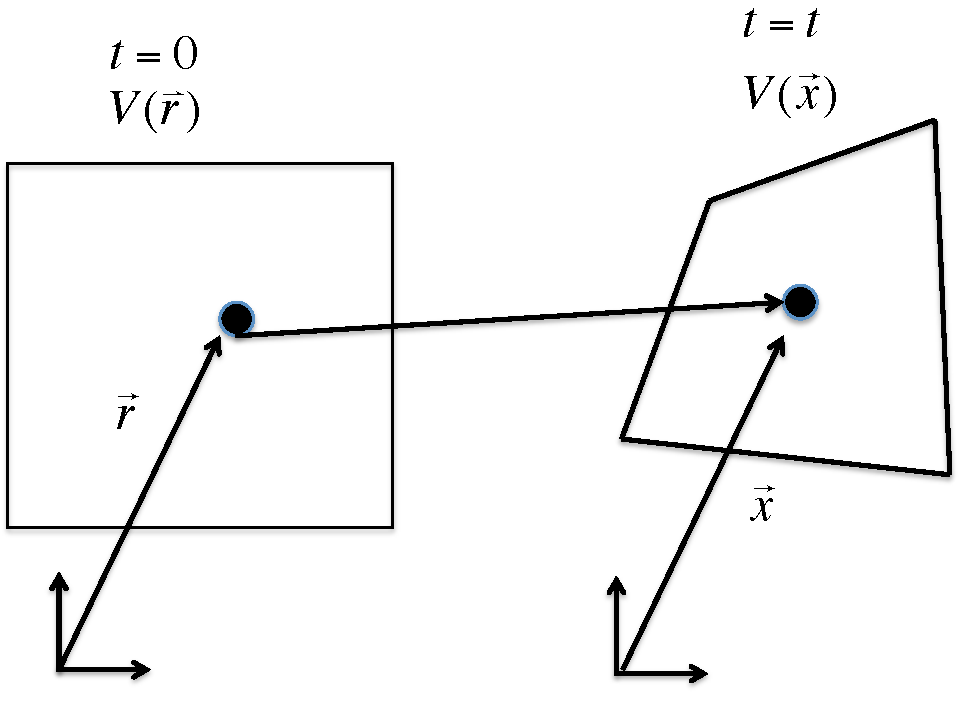
\includegraphics[width=12cm]{img/figure1.pdf}
\caption{Definition of the natural domain}
\label{fig:natural domain}
\end{figure}

 

In \eqref{motion} we can understand $\vec{r}$ like a material (Lagrangian) variable and $\vec{X}$ like a spatial (or Eulerian) variable. Using the continuum mechanics analogy it is clear that the "deformation" process at the continuum level is fully characterized by the "deformation" gradient or Jacobian of the transformation \eqref{motion} and defined according to;

\begin{equation}
dX_i=\dfrac{\partial X_i}{\partial r_J}dr_J\equiv J_{iJ}dr_J
\label{gradient}
\end{equation}

where $dr_J$ and $dX_i$ represent material vectors in the original and deformed configuration. From \eqref{gradient} it is evident that the Jacobian contains all the information describing the change of the physical sub-domain with respect to the natural element. For the element integration process we will assume that every element $V(\vec{r})$ in the natural domain deforms into the physical element $V_0(\vec{X})$ thus allowing us to write typical terms like the ones in the material stiffness matrix in (22) like;

\begin{equation}
\int\limits_{V_0(\vec{X})} \hat{B}_{ij}^K(\vec{X}) C_{ijkl} \hat{B}_{kl}^P(\vec{X}) dV_0(\vec{X})\equiv \int\limits_{V_0(\vec{X})} \hat{B}_{ij}^K(\vec{r}) C_{ijkl} \hat{B}_{kl}^P(\vec{r})J dV(\vec{r})
\label{matmatrix}
\end{equation}


where we have used $dV(\vec{X})=JdV(\vec{r})$, with $J$ being the determinant of the deformation gradient and in general we transform functions between the natural and physical space making use of \eqref{motion} according to;

\begin{equation}
f(\vec{r})=F[\vec{X}(\vec{r})]
\label{funtrans}
\end{equation}

	 								
\subsubsection{Interpolation scheme}
Having identified the fact that the integration process will take place in the natural domain we will approach the interpolation process directly in this natural space.  In the case of the displacement based finite element method all the involved variables will then be obtained via interpolation of nodal displacements.  For instance, assume that a given problem variable is defined in the physical space by the tensor $\Phi_{ik...p}(\vec{X})$. The interpolated variable is then obtained like;

\begin{equation}
\Phi_{ij...p}(\vec{X})=H_{ij...p}^K(\vec{r})\hat{u}^K
\label{interpol}
\end{equation}	 						

where $\hat{u}^K$ represents a vector of nodal points displacements, see Figure \ref{fig:interpol nat dom}, and $H_{ij...p}^K(\vec{r})$ is an interpolator which keeps the tensorial character of the original physical variable $\Phi_{ik...p}(\vec{X})$   and where the super-index makes reference to a nodal identifier and the summation convention applies.


\begin{figure}[h]
\centering
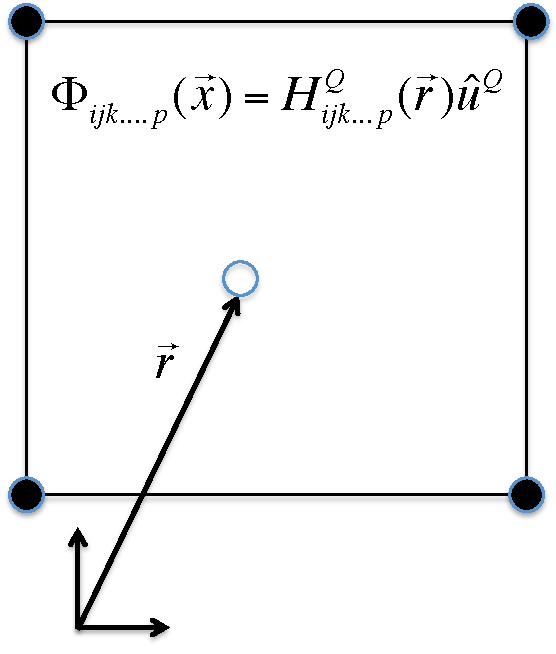
\includegraphics[width=6cm]{img/figure2.pdf}
\caption{General interpolation strategy in the natural domain}
\label{fig:interpol nat dom}
\end{figure}
 


Since the primary variable corresponds to displacements it must be kept in mind that $H_{ij...p}^K(\vec{r})$ corresponds to combinations of derivatives (or other arbitrary combinations) of the basic element shape functions defined in;


\begin{equation}
u_i(\vec{X})=N_i^K(\vec{r})\hat{u}^K
\label{el interpol}
\end{equation}



For the general interpolation process we need two kinds of transformations.  First we need to transform integrals over the physical space into integrals into the natural space which corresponds to;


\begin{equation}
\int\limits_{V_0(\vec{X})} F(\vec{X})dV_0(\vec{X})\equiv \int\limits_{V_0(\vec{r})} f(\vec{r})J dV(\vec{r})
\label{gen trans}
\end{equation}



Second we need to relate spatial differentiation in both, the physical and spatial domains.  Let us define these operators like $\bigtriangledown_i^X$ and $\bigtriangledown_I^r$ respectively. It then follows from \eqref{funtrans} and the chain rule of differentiation that;

\begin{equation}
\dfrac{\partial F}{\partial X_i}=\dfrac{\partial f}{\partial r_J}\dfrac{\partial r_J}{\partial X_i}
\label{chain}
\end{equation}

from where we can establish the connection between the two operators like


\begin{equation}
\bigtriangledown_i^X=J_{Ji}^{-1}\bigtriangledown_I^r
\label{fundamental}
\end{equation}

We further define the fundamental interpolator giving rise to gradients of the primary displacement variable in the physical space according to;


\begin{equation}
u_{i,j}(\vec{X})=L_{ij}^K(\vec{r})\hat{u}^K
\label{fund operator}
\end{equation}


This fundamental interpolator  $L_{ik}^K(\vec{r})$ is derived after using \eqref{el interpol} and \eqref{fundamental} in the physical displacement gradient definition as shown next;


\[
\begin{aligned}
u_{i,j}(\vec{X})&=\bigtriangledown_j^X u_i(\vec{X})\\
u_{i,j}(\vec{X})&=\bigtriangledown_j^X N_i^K(\vec{r})\hat{u}^K\\
u_{i,j}(\vec{X})&=J_{Qj}^{-1}\bigtriangledown_Q^r N_i^K(\vec{r})\hat{u}^K\\
u_{i,j}(\vec{X})&=J_{Qj}^{-1}N_{i,Q}^K(\vec{r})\hat{u}^K
\end{aligned}
\]

then

\begin{equation}
L_{ij}^K(\vec{r})=J_{Qj}^{-1}N_{i,Q}^K(\vec{r})
\label{fundamental interpolator}
\end{equation}

\subsubsection{Elemental stiffness matrix}
The elemental material stiffness matrix computed in the natural domain of Figure A3 reads;



\begin{equation}
K^{KP}=\int\limits_{V_0(\vec{r})} \hat{B}_{ij}^K(\vec{r}) C_{ijkl} \hat{B}_{kl}^P(\vec{r})J dV(\vec{r})\equiv \int\limits_{r=-1}^{r=+1}\int\limits_{s=-1}^{s=+1} \hat{B}_{ij}^K(r,s) C_{ijkl} \hat{B}_{kl}^P(r,s)J(r,s) \mathrm{d}r\mathrm{d}s
\label{elematrix}
\end{equation}



\begin{figure}[h]
\centering
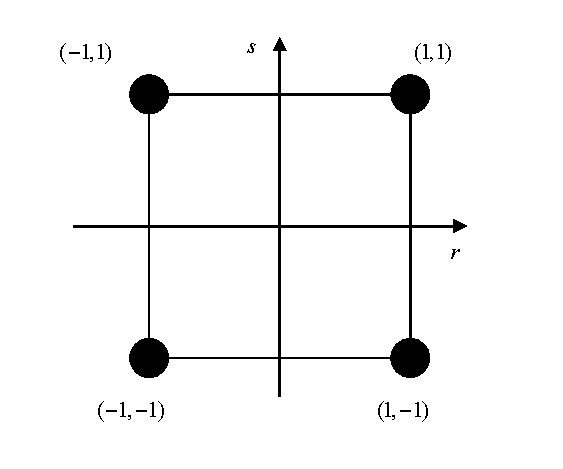
\includegraphics[width=12cm]{img/figure3.pdf}
\caption{Natural domain of integration}
\label{fig:Nat domain}
\end{figure}	 		
 

Once the interpolator $\hat{B}_{ij}^K(\vec{r})$ has been identified the elemental stiffness matrix is obtained via numerical integration (quadrature) as described in \eqref{elematrix};

\begin{equation}
\int\limits_{r=-1}^{r=+1}\int\limits_{s=-1}^{s=+1} \hat{B}_{ij}^K(r,s) C_{ijkl} \hat{B}_{kl}^P(r,s)J(r,s) \mathrm{d}r\mathrm{d}s\approx \sum_{i,j=1}^{NGPTS} \alpha_i \alpha_j \hat{B}_{kl}^K(r_i,s_j)C_{ijkl} \hat{B}_{kl}^P(r_i,s_j) J(r_i,s_j)
\label{eleinetgration}
\end{equation}

	 													(A13)

and where NGPTS corresponds to the number of integration points, $\alpha_j$ is a weighting factor and $r_i,s_j$   are the coordinates of a typical point $\vec{r}$ in the natural space of Figure A4 .

 
 \begin{figure}[h]
\centering
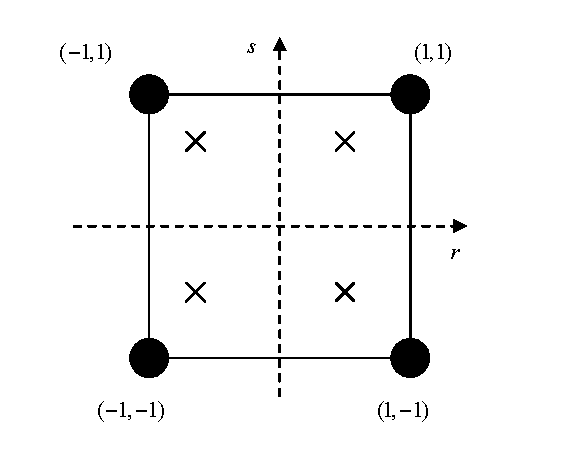
\includegraphics[width=12cm]{img/figure4.pdf}
\caption{Natural integration domain showing quadrature evaluation nodes}
\label{fig:integration domain}
\end{figure}	 


One important aspect of the numerical integration that has to be kept in mind is accuracy.  Depending on the particularly selected integration scheme, the number of introduced integration points fixes the maximum polynomial order of the considered functions that can be integrated accurately.  In the case of the integrand in \eqref{eleinetgration}, it is clear that this order increases as the distortion of the physical element  with respect to the natural element increases.  One way of dealing with this dependency of accuracy with element distortion is to make use of adaptative integration techniques which are numerically expensive.  What is actually done in standard FEM analysis is to choose the number of quadrature points beforehand and introduce distortion related error criteria inside the code in such a way that some sort of validation is performed before the numerical integration process is started.
%Capitulo "Elastodinamica"
%
\chapter{Nonlineal Equilibrium Equations in a Finite Element Discretization}

\section{General Form}


\subsection{Newton-Raphson Scheme}


\section{Algorithm}

%Capitulo "Elastodinamica"
%
\chapter{General Discrete Form for Any Given Stress-Strain Pair}

\section{General Equations}


\subsection{}


\section{}

%Chapter "Elemental Matrices"
%
\chapter{Explicit Dynamic Analysis}

\section{Statement of the Problem}
Consider the discrete dynamic equilibrium equations at time $t$

\begin{equation}
M^{t}A+C^{t}V+K^{t}U=^{t}F
\label{equil}
\end{equation}

where $M$, $C$, $K$ are the assembled mass, damping and stiffness matrix respectively and similarly $^{t}A$, $^{t}V$, $^{t}U$, ${t}F$ are the nodal accelerations, velocities, displacements and external loads vectors at time $t$. In terms of forces \eqref{equil} can be written like;

\begin{equation}
^{t}F^I+^{t}F^D+^{t}F^s=^{t}F
\label{force equil}
\end{equation}

where $^{t}F^I$, $^{t}F^D$ and $^{t}F^s$ are inertial, damping and elastic components respectively.

Expanding the acceleration and velocity terms at time $t$ in a consistent finite central differences scheme we have;

\begin{equation}
\begin{aligned}
^{t}A&=\dfrac{1}{\Delta t^2}\left(^{t-\Delta t}U-2^{t}U+^{t+\Delta t}U\right)\\
^{t}V&=\dfrac{1}{2\Delta t}\left(-^{t-\Delta t}U+^{t+\Delta t}U\right)
\end{aligned}
\label{finitediff}
\end{equation}

Using \eqref{finitediff} in \eqref{force equil} yields;


\begin{equation}
\left(\dfrac{1}{\Delta t^2}M+\dfrac{1}{2\Delta t}C\right) ^{t+\Delta t}U=^{t}F-\left(K-\dfrac{2}{\Delta t^2}M\right) ^{t}U-\left(\dfrac{1}{\Delta t^2}M-\dfrac{1}{2\Delta t^2}C\right)^{t-\Delta t}U
\label{resequil}
\end{equation}

Redefine forces as follows
\begin{equation}
\begin{aligned}
^{j}F^I&=\dfrac{1}{\Delta t^2}M ^{j}U\\
^{j}F^D&=\dfrac{1}{2 \Delta t}C ^{j}U\\
^{j}F^S&=K ^{j}U
\end{aligned}
\label{redefine}
\end{equation}

and write \eqref{resequil} as;

\begin{equation}
^{t+\Delta t}F^I+^{t+\Delta t}F^D=^{t}F-^{t}F^s+2 ^{t}F^I-^{t-\Delta t}F^I+^{t-\Delta t}F^D
\label{force equil 2}
\end{equation}

\begin{itemize}
\item \eqref{force equil 2} is an equilibrium equation at time $t=t$ allowing to predict the displacements at time $t=t+\Delta t$ in terms of previously known values at times $t$ and $t=t-\Delta t$.

\item The equation is exact within the error introduced by the expansion used in \eqref{finitediff}.

\begin{figure}[h]
\centering
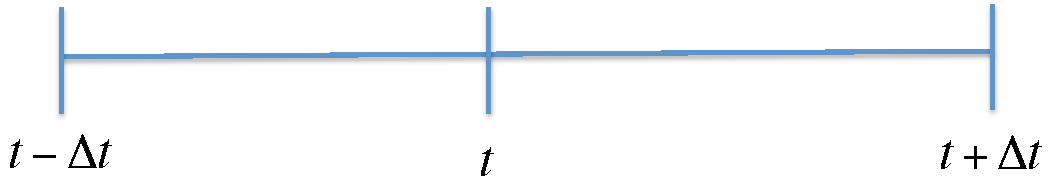
\includegraphics[width=12cm]{img/figure7_0.pdf}
\caption{Definition of the general iteration}
\label{fig:time iteration}
\end{figure}

\item The first predicted solution is at $t=\Delta t$ and we require data at $t=-\Delta t$ and at $t=0$.

\begin{figure}[h]
\centering
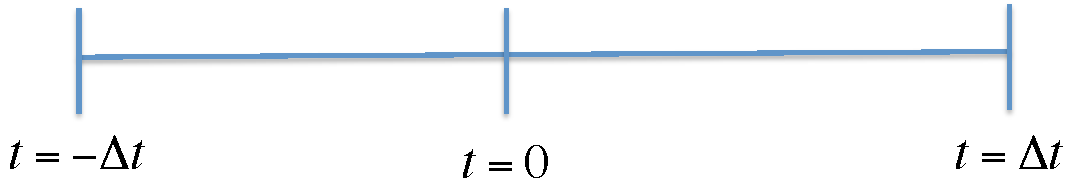
\includegraphics[width=12cm]{img/figure7_1.pdf}
\caption{Definition of the general iteration}
\label{fig:initial time iteration}
\end{figure}

\end{itemize}

\subsection{Damping Assumptions}

\begin{itemize}
\item[1] Use Rayleigh Damping and retain the velocity expansion used in \eqref{finitediff}. That is;

\begin{equation}
C=\alpha M+\beta K
\end{equation}

then we have (in terms of forces);

\begin{equation}
(1+\beta \Delta t^2) ^{t+\Delta t}F^I+\dfrac{\alpha}{2\Delta t} ^{t+\Delta t}F^S=^{t}\hat{F}
\label{Rayleigh}
\end{equation}

where;

\[
^{t}\hat{F}=^{t}R-^{t}F^S+2 ^{t}F^I-^{t-\Delta t}F^I+^{t-\Delta t}F^D
\]

Solution in equation \eqref{Rayleigh} requires the full assembly and factorization of an effective stiffness matrix.

\item[2] Neglect damping (This is however inconvenient for finite domains) 


\begin{equation}
^{t+\Delta t}F^I=^{t}F-^{t}F^S+2 ^{t}F^I-^{t-\Delta t}F^I
\label{Nodamping}
\end{equation}

\item[3] Use Rayleigh damping but modify the velocity expansion introduced in \eqref{finitediff}. Using

\begin{equation}
^{t}V=\dfrac{1}{\Delta t}(^{t}U-^{t-\Delta t}U)
\label{velocity}
\end{equation}

yielding;

\begin{equation}
^{t+\Delta t}F^I=^{t}F-^{t}F^S+2 ^{t}F^{I}-^{t}F^D+^{t-\Delta t}F^D-^{t-\Delta t}F^I
\end{equation}

Defining a set of forces associated to the initial conditions like;

\[
^{t-\Delta t}F^{IC}=^{t-\Delta t}F^I-^{t-\Delta t}F^D
\]

we have

\begin{equation}
^{t+\Delta t}F^I=^{t}F-^{t}F^S+2 ^{t}F^{I}-^{t}F^D-^{t-\Delta t}F^{IC}
\label{modvelocity}
\end{equation}

\end{itemize}

\subsection{Algorithm corresponding to the damping assumption 3}

\begin{figure}[h]
\centering
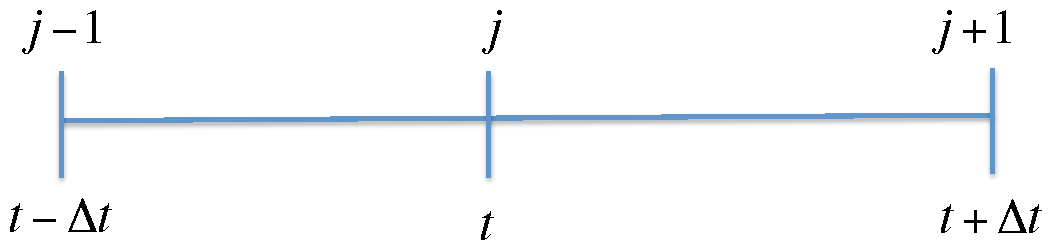
\includegraphics[width=12cm]{img/figure5.pdf}
\caption{Definition of the general iteration}
\label{fig:general iteration}
\end{figure}

Let us write \eqref{modvelocity} like

\begin{equation}
^{j+1}F^I=^{j}F-^{j}F^S+2 ^{j}F^{I}-^{j}F^D-^{j-1}F^{IC}
\label{modveliter}
\end{equation}

where the initialization process corresponds to;


\begin{figure}[h]
\centering
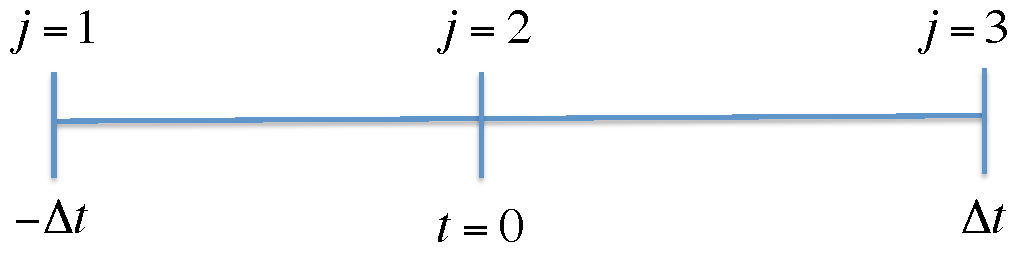
\includegraphics[width=12cm]{img/figure6.pdf}
\caption{Definition of the initial iteration}
\label{fig:initial iteration}
\end{figure}

Applying \eqref{modveliter} for $t=0$ we have;

\[
^{0}F^I=^{0}F-^{0}F^S+2 ^{0}F^{I}-^{0}F^D-^{-\Delta t}F^{IC}
\]

from which it is clear that we require $-^{\Delta t}U$. Applying the central difference expansion at $t=0$ and solving for $-^{\Delta t}U$ yields;

\begin{equation}
^{-\Delta t}U=^{0}F-\Delta t ^{0}V+\dfrac{\Delta t^2}{2} ^{0}A
\label{initialU}
\end{equation}

Using \eqref{initialU} in \eqref{modveliter} allows us to start up the algorithm.

\subsubsection{Particulars}
In what follows we concentrate on this last algorithm and in order to study some details we return to its standard displacements form. Writing \eqref{modveliter} in terms of displacements and re-arranging yields;


\begin{equation}
\dfrac{1}{\Delta t^2}M ^{t+\Delta t}U=^{t}F-(1+\dfrac{\beta}{\Delta t})K ^{t}U+(\dfrac{2}{\Delta t^2}-\dfrac{\alpha}{\Delta t})M ^{t}U-(\dfrac{1}{\Delta t^2} - \dfrac{\alpha}{\Delta t})M ^{t-\Delta t}U+(\dfrac{\beta}{\Delta t}) K ^{t-\Delta t}U
\label{disequil}
\end{equation}

Let;


\[
\begin{aligned}
a_1&=1+\dfrac{\beta}{\Delta t}\\
a_2&=\dfrac{2}{\Delta t^2}-\dfrac{\alpha}{\Delta t}\\
a_3&=\dfrac{1}{\Delta t^2} - \dfrac{\alpha}{\Delta t}\\
a_4&=\dfrac{\beta}{\Delta t}
\end{aligned}
\]


\begin{equation}
^{t+\Delta t}F^I=^{t}F-a_1K ^{t}U+a_2M ^{t}U-a_3M ^{t-\Delta t}U+a_4K ^{t-\Delta t}U
\label{equliassum3}
\end{equation}


\subsection{Decoupling}
Consider the equation for the $i$-th d.o.f;

\begin{equation}
\dfrac{1}{\Delta t^2}M_{ij} ^{t+ \Delta t}U_j=^{t}F_i-a_1K_{ij} ^{t}U_j+a_2M_{ij}^{t}U_j-a_3M_{ij} ^{t-\Delta t}U_j+a_4K_{ij}^{t-\Delta t}U_j
\label{equildecoupled1}
\end{equation}

where we keep $i$ fixed in \eqref{equildecoupled1}. For a lumped mass matrix we can write;

\[
M_{ij}=m_I\delta_{ij}
\]

then \eqref{equildecoupled1} becomes;

\begin{equation}
\dfrac{1}{\Delta t^2}m_I ^{t+ \Delta t}U_i= ^{t}F_I-a_1 K_{ij} ^{t}U_j+a_2 m_I ^{t}U_i-a_3 m_I ^{t-\Delta t} U_i+a_4 K_{ij} ^{t-\Delta t} U_j
\label{equildecoupled2}
\end{equation}

Let;

\begin{equation}
\begin{aligned}
^{t+\Delta t} F_i^I&=\dfrac{1}{\Delta t^2} m_{I} ^{t+\Delta t}U_i\\
^{t} \hat{F}^S_i&=a_1 K_{ij} ^{t}U_j\\
^{t}\hat{F}_i^I&=a_2m_{I} ^{t}U_i\\
^{t-\Delta t}\hat{F}_i^I&=a_3m_{I} ^{t-\Delta t}U_i\\
^{t-\Delta t}\hat{F}_i^S&=a_4K_{ij}^{t-\Delta t}U_j
\end{aligned}
\label{forces2}
\end{equation}

so the recursive equation takes the form;

\begin{equation}
^{t+\Delta t} F_i^I=^{t}F_i-^{t} \hat{F}^S_i+^{t}\hat{F}_i^I-^{t-\Delta t}\hat{F}_i^I+^{t-\Delta t}\hat{F}_i^S
\label{forces3}
\end{equation}

and the algorithm then reduces to;

\begin{algorithm}[H]
\SetAlgoLined
\KwData{Time span, Geometry, Material Paramters}
\KwResult{Displacements, Velocity and Acceleration time histories }
Compute $^{t+\Delta t} F_i^I$\\
Solve for $^{t+\Delta t}U_i=\left(\dfrac{\Delta t^2}{m_I}\right) ^{t+\Delta t}F_{i}^I$\\
Update $^{t}V_i$, $^{t}A_i$
\caption{Summarized Algorithm}
\end{algorithm}

To initialize the algorithm we apply the FD's equations at $t=0$

\[
\dfrac{1}{\Delta t^2}m_I ^{\Delta t}U_i=^{0}F_i-a_1 K_{ij} ^{0}U_j+a_2 m_I ^{0}U_i-a_3 m_I ^{-\Delta t} U_i+a_4 K_{ij} ^{-\Delta t} U_j
\]

where $^{-\Delta t} U_i$ is obtained from \eqref{initialU}

\begin{equation}
^{-\Delta t}U_i=^{0}U_i-\Delta t ^{0}V_i+\dfrac{\Delta t^2}{2} ^{0}A_i
\label{initialU2}
\end{equation}

The initial acceleration is obtained after assuming homogeneous IC's;

\[
m_{I} ^{0}A_i+C_{ij} ^{0}V_j +K_{ij} ^{0}U_j=^{0}F_i
\]

therefore

\[
\begin{aligned}
m_{I} ^{0}A_i=\dfrac{^{0}F_i}{m_I}\\
^{-\Delta t} U_i=\dfrac{\Delta t^2}{2m_I}^{0}F_i
\end{aligned}
\]

Moreover, neglecting the damping effects on the prediction of $^{\Delta t}U_i$ yields;

\[
^{\Delta t} U_i=\dfrac{\Delta t^2}{2m_I}^{0}F_i
\]

\begin{algorithm}[H]
 \SetAlgoLined
 \KwData{Time span, Geometry, Material Paramters}
 \KwResult{Displacements, Velocity and Acceleration time histories }
 Initialize solution vectors ($j=1$)\;
 $^{0}U_i\longrightarrow ^{1}U_i=0$, $^{0}V_i=0$, $^{1}A_i=\dfrac{^{1}R_i}{m_I}$ \;
 Select $\Delta t$ and integration constants $a_1$,$a_2$, $a_3$, $a_4$\;
 Fix 1-st predicted value (let $j=2$)\;
 \[
^{\Delta t} U_i \longleftarrow \dfrac{\Delta t^2}{2m_I} ^{0}F_i\longleftrightarrow \left[^{2}U_i \longleftarrow\dfrac{\Delta t^2}{2m_I} ^{1}F_i \right]
 \]
Time Integration Phase\;
\While{$j \leq N$}{
\[
\begin{aligned}
^{j+1}F^I_i\longleftarrow& ^{j}F_i-a_1 K_{ij} ^{j}U_j+a_2 m_I ^{j}U_j-a_3 m_I ^{j-1} U_i+a_4 K_{ij} ^{j-1} U_j\\
 ^{j+1}U_i\longleftarrow&\dfrac{\Delta t^2}{2m_I} ^{0}F^I_i\\
 ^{j}A_i\longleftarrow&\dfrac{1}{\Delta t^2}\left(^{j-1}U_i-2^{j}U_i+^{j+1}U_i\right)\\
 ^{j}V_i\longleftarrow&\dfrac{1}{2\Delta t}\left(-^{j-1}U_i+^{j+1}U_i\right)\\
 j\longleftarrow&j+1
\end{aligned}
\]
}
\caption{Full Algorithm}
\end{algorithm}

\subsubsection{Nodal Assembler}
In the uncoupled explicit finite element formulation the equation solving process proceeds one degree of freedom at a time. This implies a different assembly process to the one used in an implicit algorithm where a formal coefficient matrix is assembled and inverted. Now the mass, damping and stiffness elemental matrices are used to obtain effective nodal forces at each degree of freedom. In summary the mesh is not covered in an element by element basis, but in a node by node basis. In the following algorithm we discuss this nodal assembly process where in order to solve the displacement at a given degree of freedom prior knowledge of the element contributing to the given node is necessary. In the nodal assembler algorithm the following arrays are needed.

\noindent
ILIST(): Stores the elements connected to the current node.\\
LPLIST():Stores the local position of the current node in each one of the elements of ILIST().\\
NIEL():Number of elements at the current node. This array is used to access ILIST().\\


\begin{algorithm}[H]
\SetAlgoLined
\KwData{Number of nodal points, number of elements, Model}
\KwResult{Displacements, Velocity and Acceleration time histories }
\While {$i \leq NUMNP$}
{
$K\leftarrow NIEL(i)$
%\while {$ik \leq 2$}{
%$jK \leftarrow ID(ik,i)$
%}
}
\caption{Nodal Assembler}
\end{algorithm}







%%%%%%%%%%%%%%%%%%%%%%%%%%%%%%%%%%%%%%%%%%%%%%%%%%%%%%%%%%%%%%%%%%%%%%%%%%%%
%%%%%% Bibliografia %%%%%%%%%%
%%Para referenciar sin cita en el texto
%\nocite{}
\addcontentsline{toc}{chapter}{Referencias}
\bibliographystyle{babunsrt}
%\bibliography{informe}

%%%%%%%%%%%%%%%%%%%%%%%%%%%%%%%%%%%%%%%%%%%%%%%%%%%%%%%%%%%%%%%%%%%%%%%%%%%%

\end{document}

